\chapter{\ac{API}s}\label{ch:apis}
In diesem Kapitel wird detaillierter auf die Verwendung von verschiedenen \ac{API}s in unserem 
Projekt eingegangen.

\section{Guidelines}
In dieses Projekt orientiert sich in Bezug auf \ac{API}s an den Zalando API 
Guidelines\footnote{https://opensource.zalando.com/restful-api-guidelines/}.
Diese werden, so weit sie für das Projekt förderlich und sinnvoll sind, bei der Implementierung
berücksichtigt.

\section{Verwendete \ac{API}s}
Um Daten in unserer Datenbank zu speichern und abzufragen, wird die OpenAPI Specification
verwendet. Diese bietet die Möglichkeit, die Integration der verschiedenen Bestandteile der
\ac{API}, nach den Zalando Guidelines automatisch, auf Basis einer im \Gls{yaml} Format hinterlegten
Beschreibung der gewünschten \ac{API}, zu generieren. So kann Fehlern im Development
Prozess vorgebeugt und der Prozess an sich beschleunigt werden.

\section{Endpoints}
Folgende Endpunkte sind in der verwendeten \ac{API}, mit Hilfe eines gültigen Bearer Tokens, ansprechbar. 

\subsection{GET /templates}

Dieser \ac{API} Endpunkt liefert alle in der Datenbank gespeicherten Templates zurück. Diese
werden genutzt, um die Buttons auf der Main Page dynamisch zu generieren. Da hierfür nicht
alle Informationen über die Templates benötigt werden, sind in der Antwort nicht alle
Informationen über die einzelnen Templates enthalten.

\subsection{GET /templates/{templateId}}
Dieser Endpunkt gibt ein bestimmtes Template zurück. Im Vergleich zum Ergebnis des vorherigen
Endpunkts werden jedoch deutlich mehr Details zurückgegeben.

\section{Schemata}
Im Folgenden werden die verwendeten Schemata grob beschrieben. Für detailliertere Informationen
wird auf \ref{sec:Detailiertere Informationen} verwiesen.

\subsection{FormElement}
Das FormElement Schema beinhaltet alle Daten, die für ein einzelnes, dynamisch generiertes
Eingabeelement benötigt wird.

\subsection{FormSection}
Das Schema der FormSection beinhaltet Daten, die für die dynamische Generierung einer Sektion
für das Ausfüllen eines Antrags, benötigt werden. Dazu zählt eine Liste der FormElements in
dieser Section, sowie eine Reihenfolge, um die Sections ordnen zu können.

\subsection{Attachment}
Das Attachment Schema dient der Organisation und Ordnung der dem Antrag beigefügten Dateien.

\subsection{Form}
Das Form Schema entspricht in seinen Daten, einem kompletten Antrag und besteht aus mehreren
FormSections, die wiederum aus mehreren FormElements bestehen, sowie potenziellen Attachments.

\section{Detailierte Informtionen}\label{sec:Detailiertere Informationen}
Im Folgenden ist der exakte Aufbau der Endpunkte und der Schemata unserer \ac{API} dokumentiert.
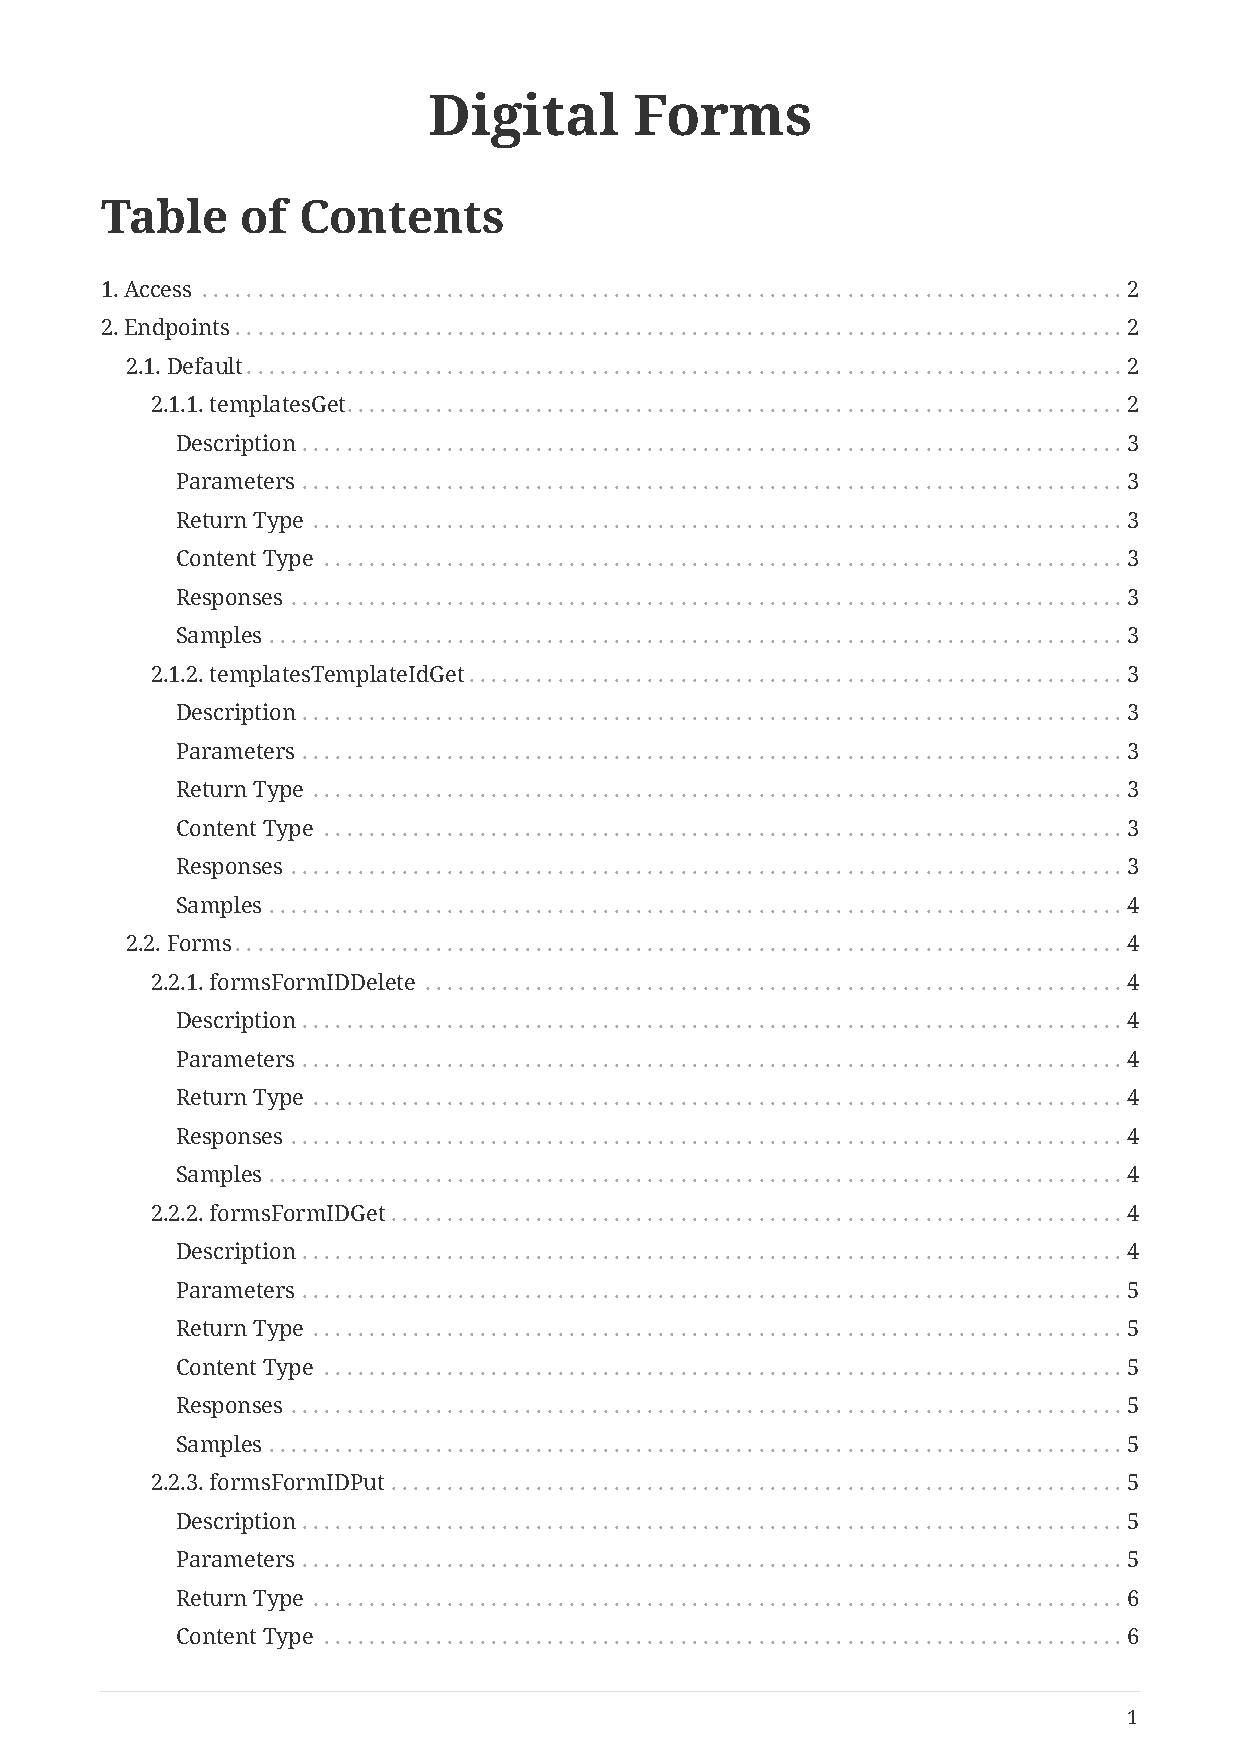
\includepdf[pages=-, landscape=true]{API_Spec.pdf}